\documentclass[14pt]{extbook}
\usepackage{multicol, enumerate, enumitem, hyperref, color, soul, setspace, parskip, fancyhdr} %General Packages
\usepackage{amssymb, amsthm, amsmath, latexsym, units, mathtools} %Math Packages
\everymath{\displaystyle} %All math in Display Style
% Packages with additional options
\usepackage[headsep=0.5cm,headheight=12pt, left=1 in,right= 1 in,top= 1 in,bottom= 1 in]{geometry}
\usepackage[usenames,dvipsnames]{xcolor}
\usepackage{dashrule}  % Package to use the command below to create lines between items
\newcommand{\litem}[1]{\item#1\hspace*{-1cm}\rule{\textwidth}{0.4pt}}
\pagestyle{fancy}
\lhead{Progress Quiz 6}
\chead{}
\rhead{Version B}
\lfoot{4563-7456}
\cfoot{}
\rfoot{Summer C 2021}
\begin{document}

\begin{enumerate}
\litem{
Graph the equation below.\[ f(x) = (x+1)^2 - 10 \]\begin{enumerate}[label=\Alph*.]
\begin{multicols}{2}\item 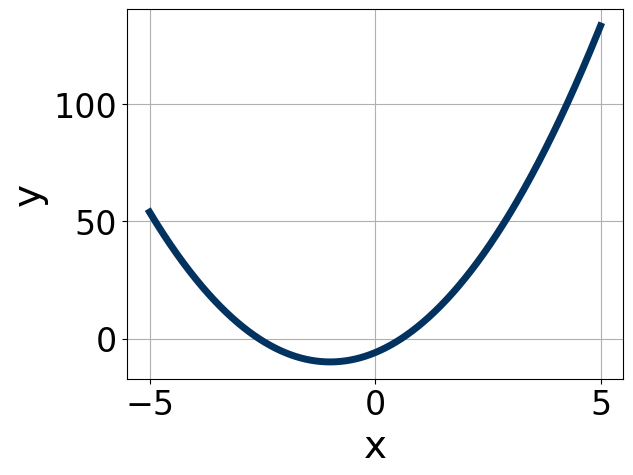
\includegraphics[width = 0.3\textwidth]{../Figures/quadraticEquationToGraphCopyAB.png}\item 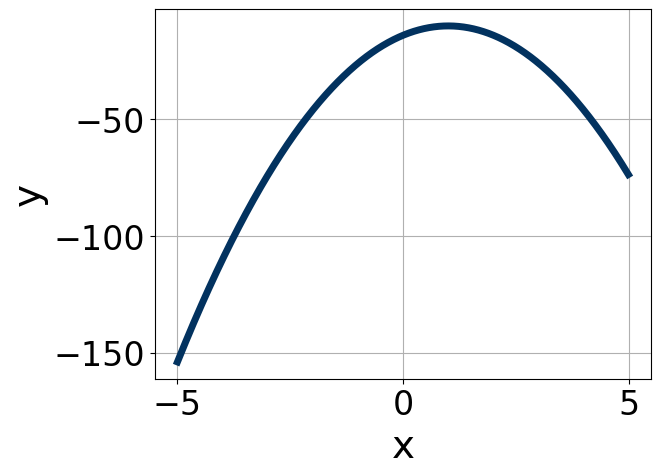
\includegraphics[width = 0.3\textwidth]{../Figures/quadraticEquationToGraphCopyBB.png}\item 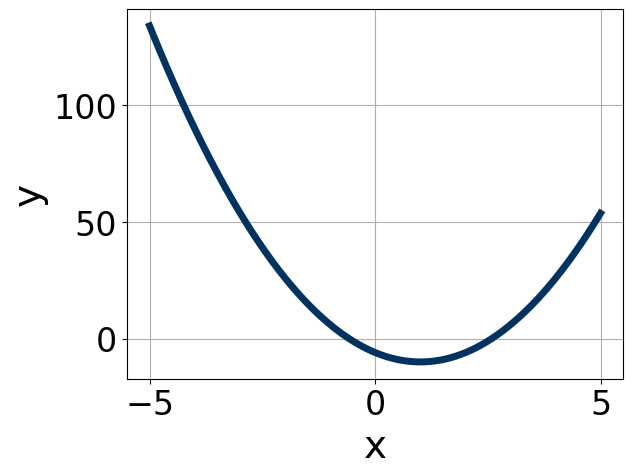
\includegraphics[width = 0.3\textwidth]{../Figures/quadraticEquationToGraphCopyCB.png}\item 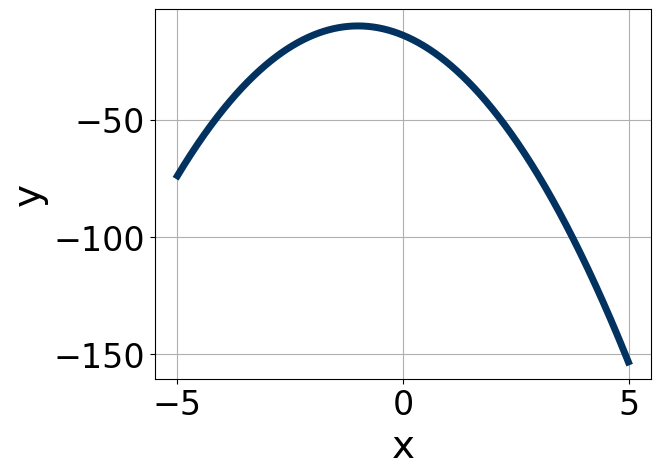
\includegraphics[width = 0.3\textwidth]{../Figures/quadraticEquationToGraphCopyDB.png}\end{multicols}\item None of the above.
\end{enumerate} }
\litem{
Factor the quadratic below. Then, choose the intervals that contain the constants in the form $(ax+b)(cx+d); b \leq d.$\[ 36x^{2} +60 x + 25 \]\begin{enumerate}[label=\Alph*.]
\item \( a \in [5.5, 6.7], \hspace*{5mm} b \in [4, 10], \hspace*{5mm} c \in [4.4, 7.1], \text{ and } \hspace*{5mm} d \in [5, 10] \)
\item \( a \in [-1.8, 1.6], \hspace*{5mm} b \in [28, 34], \hspace*{5mm} c \in [0.7, 2.5], \text{ and } \hspace*{5mm} d \in [28, 31] \)
\item \( a \in [10.3, 14.2], \hspace*{5mm} b \in [4, 10], \hspace*{5mm} c \in [1.1, 4.7], \text{ and } \hspace*{5mm} d \in [5, 10] \)
\item \( a \in [1.1, 4.1], \hspace*{5mm} b \in [4, 10], \hspace*{5mm} c \in [11.7, 12.4], \text{ and } \hspace*{5mm} d \in [5, 10] \)
\item \( \text{None of the above.} \)

\end{enumerate} }
\litem{
Factor the quadratic below. Then, choose the intervals that contain the constants in the form $(ax+b)(cx+d); b \leq d.$\[ 24x^{2} +50 x + 25 \]\begin{enumerate}[label=\Alph*.]
\item \( a \in [-0.9, 2.5], \hspace*{5mm} b \in [16, 22], \hspace*{5mm} c \in [0.8, 1.14], \text{ and } \hspace*{5mm} d \in [30, 34] \)
\item \( a \in [5.3, 8.8], \hspace*{5mm} b \in [5, 11], \hspace*{5mm} c \in [3.86, 4.62], \text{ and } \hspace*{5mm} d \in [4, 9] \)
\item \( a \in [9.4, 14.1], \hspace*{5mm} b \in [5, 11], \hspace*{5mm} c \in [1.84, 2.09], \text{ and } \hspace*{5mm} d \in [4, 9] \)
\item \( a \in [2.9, 3.4], \hspace*{5mm} b \in [5, 11], \hspace*{5mm} c \in [4.77, 8.57], \text{ and } \hspace*{5mm} d \in [4, 9] \)
\item \( \text{None of the above.} \)

\end{enumerate} }
\litem{
Graph the equation below.\[ f(x) = -(x-2)^2 + 10 \]\begin{enumerate}[label=\Alph*.]
\begin{multicols}{2}\item 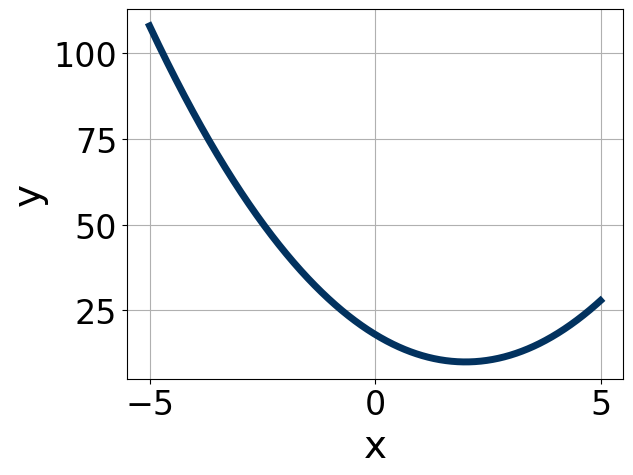
\includegraphics[width = 0.3\textwidth]{../Figures/quadraticEquationToGraphAB.png}\item 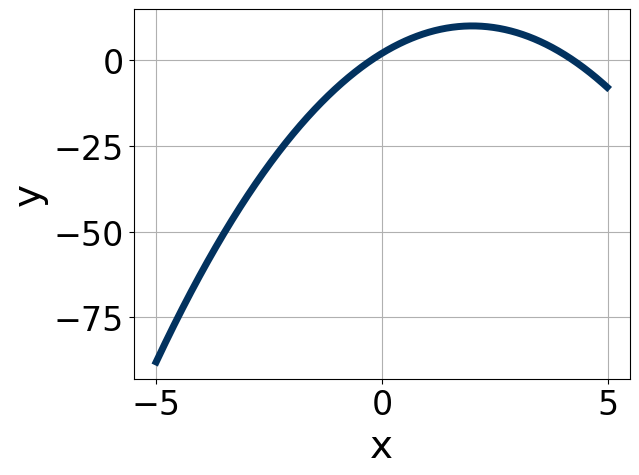
\includegraphics[width = 0.3\textwidth]{../Figures/quadraticEquationToGraphBB.png}\item 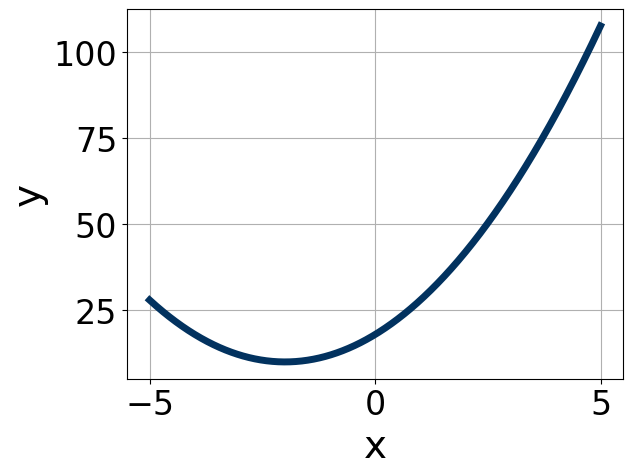
\includegraphics[width = 0.3\textwidth]{../Figures/quadraticEquationToGraphCB.png}\item 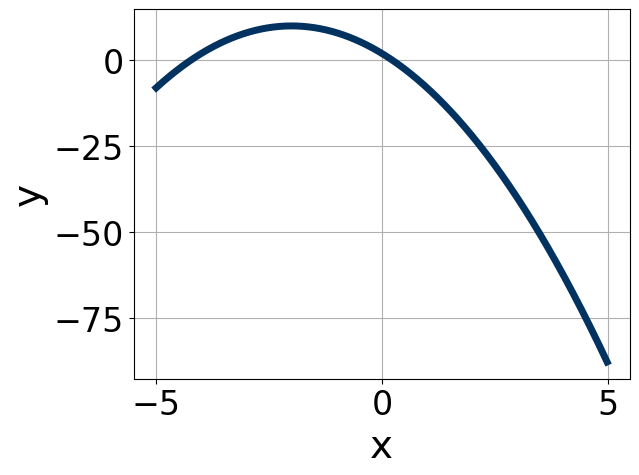
\includegraphics[width = 0.3\textwidth]{../Figures/quadraticEquationToGraphDB.png}\end{multicols}\item None of the above.
\end{enumerate} }
\litem{
Solve the quadratic equation below. Then, choose the intervals that the solutions belong to, with $x_1 \leq x_2$ (if they exist).\[ -15x^{2} +14 x + 4 = 0 \]\begin{enumerate}[label=\Alph*.]
\item \( x_1 \in [-18.23, -17.35] \text{ and } x_2 \in [2.3, 5.3] \)
\item \( x_1 \in [-20.79, -19.67] \text{ and } x_2 \in [20.9, 21.4] \)
\item \( x_1 \in [-0.95, -0.13] \text{ and } x_2 \in [0.9, 1.9] \)
\item \( x_1 \in [-1.63, -0.76] \text{ and } x_2 \in [-0.8, 1] \)
\item \( \text{There are no Real solutions.} \)

\end{enumerate} }
\litem{
Solve the quadratic equation below. Then, choose the intervals that the solutions belong to, with $x_1 \leq x_2$ (if they exist).\[ 20x^{2} -12 x -4 = 0 \]\begin{enumerate}[label=\Alph*.]
\item \( x_1 \in [-2.8, -0.6] \text{ and } x_2 \in [-0.14, 0.51] \)
\item \( x_1 \in [-6.1, -3.5] \text{ and } x_2 \in [16.46, 17.17] \)
\item \( x_1 \in [-22.6, -21] \text{ and } x_2 \in [21, 22.99] \)
\item \( x_1 \in [-0.8, 0.1] \text{ and } x_2 \in [0.73, 0.88] \)
\item \( \text{There are no Real solutions.} \)

\end{enumerate} }
\litem{
Solve the quadratic equation below. Then, choose the intervals that the solutions $x_1$ and $x_2$ belong to, with $x_1 \leq x_2$.\[ 10x^{2} -53 x + 36 = 0 \]\begin{enumerate}[label=\Alph*.]
\item \( x_1 \in [0.32, 0.5] \text{ and } x_2 \in [8.64, 9.16] \)
\item \( x_1 \in [7.96, 8.19] \text{ and } x_2 \in [44.81, 45.46] \)
\item \( x_1 \in [0.71, 0.83] \text{ and } x_2 \in [4.25, 5.03] \)
\item \( x_1 \in [0.81, 0.92] \text{ and } x_2 \in [3.77, 4.23] \)
\item \( x_1 \in [1.5, 1.82] \text{ and } x_2 \in [1.57, 3] \)

\end{enumerate} }
\litem{
Solve the quadratic equation below. Then, choose the intervals that the solutions $x_1$ and $x_2$ belong to, with $x_1 \leq x_2$.\[ 15x^{2} +38 x + 24 = 0 \]\begin{enumerate}[label=\Alph*.]
\item \( x_1 \in [-2.19, 0.62] \text{ and } x_2 \in [-1.26, -1.2] \)
\item \( x_1 \in [-3.17, -1.5] \text{ and } x_2 \in [-0.82, -0.45] \)
\item \( x_1 \in [-5.27, -3.33] \text{ and } x_2 \in [-0.41, -0.32] \)
\item \( x_1 \in [-6.8, -5.15] \text{ and } x_2 \in [-0.33, -0.24] \)
\item \( x_1 \in [-20.47, -19.44] \text{ and } x_2 \in [-18.02, -17.91] \)

\end{enumerate} }
\litem{
Write the equation of the graph presented below in the form $f(x)=ax^2+bx+c$, assuming  $a=1$ or $a=-1$. Then, choose the intervals that $a, b,$ and $c$ belong to.
\begin{center}
    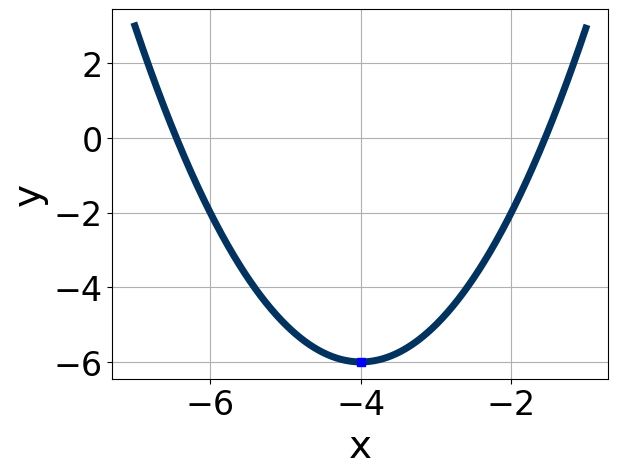
\includegraphics[width=0.5\textwidth]{../Figures/quadraticGraphToEquationB.png}
\end{center}
\begin{enumerate}[label=\Alph*.]
\item \( a \in [1, 2], \hspace*{5mm} b \in [6, 13], \text{ and } \hspace*{5mm} c \in [8, 11] \)
\item \( a \in [-3, 0], \hspace*{5mm} b \in [6, 13], \text{ and } \hspace*{5mm} c \in [-25, -19] \)
\item \( a \in [-3, 0], \hspace*{5mm} b \in [-10, -6], \text{ and } \hspace*{5mm} c \in [-25, -19] \)
\item \( a \in [1, 2], \hspace*{5mm} b \in [-10, -6], \text{ and } \hspace*{5mm} c \in [22, 26] \)
\item \( a \in [1, 2], \hspace*{5mm} b \in [-10, -6], \text{ and } \hspace*{5mm} c \in [8, 11] \)

\end{enumerate} }
\litem{
Write the equation of the graph presented below in the form $f(x)=ax^2+bx+c$, assuming  $a=1$ or $a=-1$. Then, choose the intervals that $a, b,$ and $c$ belong to.
\begin{center}
    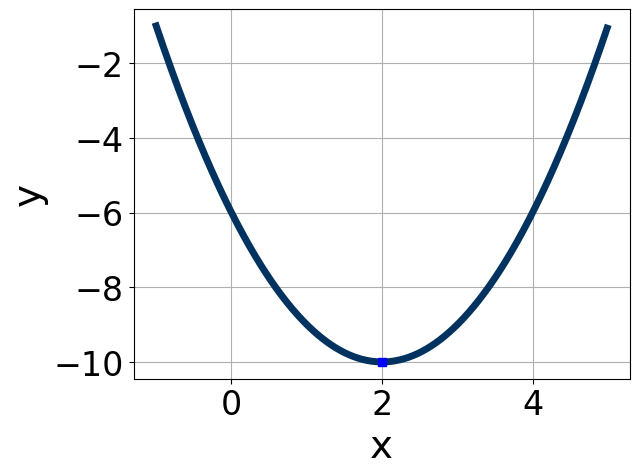
\includegraphics[width=0.5\textwidth]{../Figures/quadraticGraphToEquationCopyB.png}
\end{center}
\begin{enumerate}[label=\Alph*.]
\item \( a \in [-0.9, 1.7], \hspace*{5mm} b \in [-4, 0], \text{ and } \hspace*{5mm} c \in [-9, -4] \)
\item \( a \in [-1.7, 0.1], \hspace*{5mm} b \in [-4, 0], \text{ and } \hspace*{5mm} c \in [-14, -12] \)
\item \( a \in [-1.7, 0.1], \hspace*{5mm} b \in [3, 6], \text{ and } \hspace*{5mm} c \in [-14, -12] \)
\item \( a \in [-0.9, 1.7], \hspace*{5mm} b \in [3, 6], \text{ and } \hspace*{5mm} c \in [-9, -4] \)
\item \( a \in [-0.9, 1.7], \hspace*{5mm} b \in [3, 6], \text{ and } \hspace*{5mm} c \in [13, 15] \)

\end{enumerate} }
\end{enumerate}

\end{document}